%%%%%%%%%%%%%%%%%%%%%%%%%%%%%%%%%%%%%%%%%%%%%%%%%%%%%%%%%%%%%%%%%%%%%%%%%%%%%%%%
%2345678901234567890123456789012345678901234567890123456789012345678901234567890
%        1         2         3         4         5         6         7         8

\documentclass[letterpaper, 10 pt, conference]{IEEEconf}  % Comment this line out
                                                          % if you need a4paper
%\documentclass[a4paper, 10pt, conference]{ieeeconf}      % Use this line for a4
                                                          % paper

\IEEEoverridecommandlockouts                              % This command is only
                                                          % needed if you want to
                                                          % use the \thanks command
\overrideIEEEmargins
% See the \addtolength command later in the file to balance the column lengths
% on the last page of the document



% The following packages can be found on http:\\www.ctan.org
\usepackage{graphicx}
\usepackage{graphics} % for pdf, bitmapped graphics files
%\usepackage{epsfig} % for postscript graphics files
%\usepackage{mathptmx} % assumes new font selection scheme installed
%\usepackage{times} % assumes new font selection scheme installed
%\usepackage{amsmath} % assumes amsmath package installed
%\usepackage{amssymb}  % assumes amsmath package installed
\usepackage{hyperref}
\usepackage{textcomp}


\title{\LARGE \bf
	Object tracking with the Universal Robots\texttrademark \ UR5  
}

%\author{ \parbox{3 in}{\centering Huibert Kwakernaak*
%         \thanks{*Use the $\backslash$thanks command to put information here}\\
%         Faculty of Electrical Engineering, Mathematics and Computer Science\\
%         University of Twente\\
%         7500 AE Enschede, The Netherlands\\
%         {\tt\small h.kwakernaak@autsubmit.com}}
%         \hspace*{ 0.5 in}
%         \parbox{3 in}{ \centering Pradeep Misra**
%         \thanks{**The footnote marks may be inserted manually}\\
%        Department of Electrical Engineering \\
%         Wright State University\\
%         Dayton, OH 45435, USA\\
%         {\tt\small pmisra@cs.wright.edu}}
%}

\author{Ayla Shamineh Nawaz and Dawid Horacy Golebiewski}% <-this % stops a space
%\thanks{*This work was not supported by any organization}% <-this % stops a space
%\thanks{$^{1}$H. Kwakernaak is with Faculty of Electrical Engineering, Mathematics %and Computer Science,
%        University of Twente, 7500 AE Enschede, The Netherlands
%        {\tt\small h.kwakernaak at papercept.net}}%
%\thanks{$^{2}$D. Golebiewski is with the Department of Electrical Engineering, Hamburg University of Technology,
%        Dayton, OH 45435, USA
%        {\tt\small d.golebiewski at tuhh.de}}%
%}


\begin{document}



\maketitle
\thispagestyle{empty}
\pagestyle{empty}


%%%%%%%%%%%%%%%%%%%%%%%%%%%%%%%%%%%%%%%%%%%%%%%%%%%%%%%%%%%%%%%%%%%%%%%%%%%%%%%%
\begin{abstract}
This paper concerns a general tracking problem in which a camera is mounted on the end effector of an articulated robot (UR5). Using image processing techniques and basic kinematic ideas, a method for tracking an object on a plane is introduced and explained. The limitations and alternative approaches to this problem are outlined and treated in the discussion section.
\end{abstract}


%%%%%%%%%%%%%%%%%%%%%%%%%%%%%%%%%%%%%%%%%%%%%%%%%%%%%%%%%%%%%%%%%%%%%%%%%%%%%%%%
\section{INTRODUCTION}
Object tracking is an important part of many robotic applications. Especially in medical applicaitions the advantage of a robot being able to identify a certain object from the rest of the body and being able to not loose track of that object is high. For example surgical procedures can be augmented by using vision capabilities and sensor capabilities of robotic systems that a human surgeon by himself cannot have. To better understand the different aspects of tracking an object with a robot a simple tracking problem was adressed. A red object was placed on the same table on which the used robot arm was mounted. With the help of a camera mounted on the end effector of the robot arm, a method was implemented with which the robot arm is able to track the movement of a red test object on the table. Tracking was used in the sense of centering the object in the image plane. It is important at this point to realize that there were no other restrictions on how the robot arm should in general move through it's workspace while tracking the object. There are therefore multiple possibilities for realizing such a tracking problem. This paper provides a method for tracking in which the z-axis of the end effector is at any time oriented in the negative-z direction of the world coordinate frame. The world coordinate frame is defined as the origin of the first joint of the robot, with the z-axis being perpendicular to the table. At the same time the distance between table and the end effector is to be held constant. Since this will correspond to a motion of the robot in which the end effector is parallel to the table at all times, it is called "parallel tracking". This means that the X,Y position of the end effector is solely definded by the position of the red object. Doing so, no time has to be spent on defining possible end effector positions. This can lead to smoother and faster tracking. In the following we will present the steps necessary for parallel object tracking. This includes the kinematic properties of the robot and a way to define them for tracking purposes. As well as image processing concerning object recognition. It will be clear that most of the discussed methods also apply if a different form of tracking is chosen.

% \begin{itemize}
% \item problem discription
% \item looked at spherical tracking
% \item looked at parallel tracking
% \item red object recogintion any red object, just a dot?
% \item red object position defined
% \item position of the camera to the red object defined. e.g. our choice of tracking

% \end{itemize}

\section{Procedure and methods}

\subsection{General Setup}
The Universal Robot's UR5 model is a general-purpose articulated robot built using 6 serially connected rotary joints. It has a TCP/IP network interface and the MTEC institute at TUHH provided us with a MATLAB interface to connect with the robot's internal server, send commands and receive all information about the current state of the UR5. Attached to UR5's end effector was a Logitech QuickCam Pro 9000, which we chose to use at the maximum resolution of 1600x1200 pixels. The connection was direct over USB 2.0. 
To have tracking capability as close to real-time as possible the entire processing chain should be as fast as possible - ideally, the position of the camera center would only lag behind the object location by the image processing time $t_{img}$, the delay to calculate the target pose $t_{pos}$, the delay of getting the current state of the robot $t_{sta}$ and sending the next position $t_{snd}$ to the UR5. The sum of these variables is the variable reaction time $t_{chain}$. Knowing that the camera has a maximum frame rate of only 5 fps at its maximum resolution, we can deduce that the update frequency of our tracking setup is $5 $ Hz, since the image processing is parallel to the kinematics of the robot and a new pose is computed (if necessary) each time a frame from he video stream is acquired. This means that for large changes in target position, that result in $t_{move} > t_{FPS} $ the movement exectued by the UR5 can be interrupted by an updated target pose, which is an important feature for our intended use. %The total time-to-target position would be $ t_{FPS}+t_{chain}+t_{move} $, if the notion of a continuously moving target is abandoned.
\subsection{Kinematics and Inverse Kinematics}
Kinematic as well as Inverse Kinematic principals are used to relate the pose of the end effector to the world coordinate system and vice versa. Provided with the joint parameters of the robot, the relationships are described through simple transformation matrices. The transformation matrix from end effector of the robot to the base is described by a matrix filled with the information of the Denavit Hartenberg parameters and is only dependent on the joint parameters. Since the base of the robot and the base of the world coordinate system coincide this transformation matrix is just the pose of the end effector for a given set of joint parameters. Inverse kinematics is useful when the target pose of the end effector is computed and the joint parameters that are sent to the robot have to be determined. For each pose there are more than one possible solution set of joint parameters. The relationship between camera and end effector, also represented by a transformation matrix $H_{cam2endeff}$ will be computed once and will not change during tracking. This relationship can be determined through hand to eye calibration as explained in the following.
\subsection{Camera calibration}
Camera calibration is a method to estimate the intrinsic  parameters of the camera such as focal point, image sensor format, and principal point. This information is collected in a matrix (intrinsicparam). It also includes the estimation of the extrinsic parameters such as the transformation matrix from world coordinates to camera coordinates. The hand-eye calibration relating the position of the camera to the position of the end effector (Hcam2endeff) is also needed. Hand eye calibration as well as the intrinsic camera parameters can be computed using the proposed fully automatic camera and hand to eye calibration with a MATLAB add-on package. This package requires a certain amount of pictures taken by the camera of a grid that can be also be downloaded from \url{https://www.vision.ee.ethz.ch/software/calibration_toolbox/calibration_toolbox.php}. The grid is placed on the table and the pictures are taken from different angles, providing a unique pose for each picture. Both the pictures and the poses are requirements for the toolbox to compute the camera and the hand to eye calibration simultaneously.

\subsection{Target localisation in the Image Plane}
%We assume a pinhole camera model, we know that every scene in the world results in an inverted image on the camera sensor, which defines the image plane.
The image is aquired directly from the camera so that the image data can be used directly in the MATLAB environment. The focus of the solution lies in detecting circular objects for tracking as the test object used was of circular shape. To extend the capability of the system, a more general method has been implemented: to allow for the tracking of multiple objects of non-circular shape, the center of mass of all red shapes in the image is computed. This step is illustrated in Fig.1. In order to be able to find the the red objects in the scene in the field of vision, the acquired image is processed in the following steps:
\begin{enumerate}
\item Subtract red channel from grayscale image of the acquired frame
\item Use median filter $medfilt2(scene,[3~3])$ to filter out noise
\item Convert the resulting grayscale image into a binary image using $im2bw$
\item Remove small connected areas (fewer than 100px) from the binary image using $bwareaopen(scene,100)$ (see Fig.1)
\item Label all the connected areas in the scene using $bwlabel(scene,8)$
\item Use the $regionprops$ function to do image blob analysis using Eccentricity and the Centroid of the labeled areas
\item Case distinction: 
{\setlength\itemindent{25pt} \begin{enumerate}\item{If circular shape is found, find its centroid's coordinates}\item{Else If more than one connected area present, compute coordinates of the \textbf{center of mass} of all objects adn return $x_{pixel},y_{pixel}$} \item{Return coordinates on the image plane as $x_{pixel},y_{pixel}$ in pixel units}\end{enumerate}} 
\end{enumerate}
\begin{figure}
%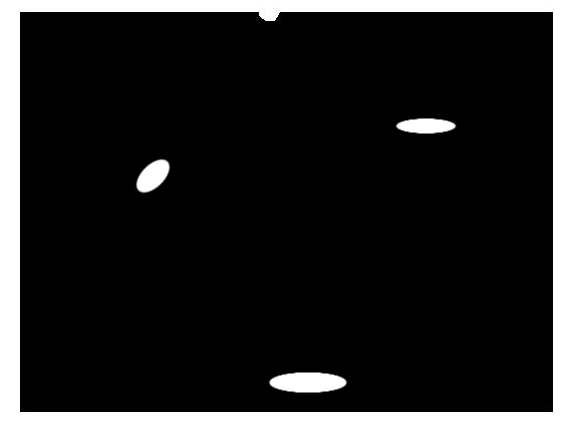
\includegraphics[width=0.5\textwidth]{daniel_suksuk.jpg}
\caption*{\label{fig:center of mass}Last step in image processing. In this case, the center of mass of all white connected areas would be computed.}
\end{figure}

%#####################################################
\subsection{Center of object in World coordinates}

The position of the red object in world coordinates is defined by the ray of the object intersecting with the principal point of the camera(see Fig.2). The direction of the negative part of the ray is given by the pixel coordinates $x_{pixel},y_{pixel}$ that were identified as the localization of the objects' centroid in the image plane. The distance of the principal point to the camera center, shown also in Fig.2. This length is the value of the focal length and can easily be extracted from the intrinsic camera parameters obtained though camera calibration. The pose of the principal point in world coordinates can be determined by the current pose of the end effector - given by the current joint parameters - and the matrix of the hand-to-eye calibration (Hcam2endeff). It is defined by: $pose*(Hcam2endeff)^{⁻1}$. Taking the principal point as the origin and going in the defined direction the $x_{world}$ and $y_{world}$ coordinates of the object can be computed with the condition that the object will always be at $z=0$.  
\begin{figure}
%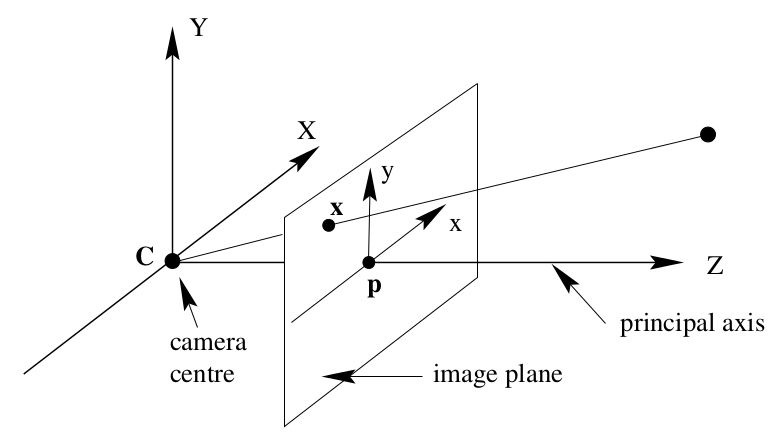
\includegraphics[width=0.5\textwidth]{DaniLLL.jpg}
\caption*{\label{fig:finding target position}ray of object on image plane}
\end{figure}

%######################################################
\subsection{Constructing the target pose of the end effector}
The target pose of the end effector is defined by the position of the object in world coordinates $x_{world}$ and $y_{world}$. Considering that the total arm length (from base to end effector) of the robot arm  is about $0.8m$, the z-coordinate can be chosen arbitrarily as long as a collision with the table is avoided. It should however be considered that when choosing the z-coordinate of the target pose too high the area which the robot can track will become smaller. On the other hand, choosing the z-coordinate too low will make it harder for the robot to track fast moving objects, since the field of vision will reduce. A height of $z=0.3m$ offered a good compromise between the field of vision an d reachable workspace in parallel mode.\\The rotation of the end effector is constructed such that the z-coordinate of the end effector will always point in the negative z direction of the world coordinate system. The remaining components of the rotation matrix were taken from a pose that was set up manually. We chose this pose in a way that the camera was aligned with the longer side of the table. Of course any other pose of the end effector is also acceptable.

%#######################################################

\subsection{Using the target pose to determine the joint parameters}

The joint parameters, as was mentioned earlier, can be found by using indirect kinematics. The solution to an indirect kinematic problem is not unique. In the case of the UR5 there are three parameters that cause the multiple solutions. These parameters reflect the fact that although the center of end effector is well defined, the robot can reach the point in different ways. This means that arm, elbow and wrist of the robot can be in either of two positions each. This leads to a solution set of 8 different possible joint solutions.
Therefore a method of choosing an adequate solution out of the provided solution set has to be defined. \\
The chosen solution for the tracking problem is the one that will keep the movement of the different links to a minimum. Define a vector diff as the difference of the current joint positions to the joint positions in the solution set. The minimum of total motion is then defined as the vector which respective diff vector has the minimal euclidean norm. 

%########################################################

\subsection{Error Handling}
To assure continuous operation error cases need to be handled. The central error that we handle is the one that happens when
the object is outside of the parallely reachable workspace, which leads to invalid solutions of the inverse kinematics. In that instance, we catch the invalid solution and define the weight of the calculated solution as infinite, so that it loses out in the minimization procedure. If \textbf{all} solultion are invalid, the is debug output to the console stating that the point is at an unreachable position. 

\section{RESULTS}

%\subsection{Object localisation in Image Plane}

Tracking of one or more red objects with the described method was implemented and tracking of a red object could be observed. As assumed, the tracking area was limited to a sub area of the reachable workspace: it is a circle which has a radius just below the maximum workspace of the robot. This is due to the fact that the decision to keep the end effector parallel to the X-Y-Plane requires the 5th joint stay fixed. Thus the last link stays vertical, which shortens the total arm length. The speed of tracking is mainly limited by the frame rate and the movment time, the processing time is negligible. For development, a speed factor of 0.05 was used. Interpreting the camera image multiple times while the robot is moving leads to a faster reaction to position changes of the red test object. On the other hand the motion of the robot becomes less smooth. Tracking will hold as long as either no red object is detected by the camera or the position of the red object is physically not reachable by the robot. 
\section{DISCUSSION}
Our tracking concept allows for tracking on a parallel plane - this is  the simpler solution from the implementational point of view, since one coordinate in world space is fixed - but the cost is the loss of 3D tracking ability. An extension to this could be achieved by using a different projection model, for instance by setting a midpoint of a virtual sphere inside the workspace and limiting the movement of the UR5's end effector to the sphere's diameter. Another well established solution is the POSIT procedure [2], which has the advantage of calculating the pose of a specific object of known dimension from a single-view camera setup. While this provided a very interesting solution to the location estimation problem, the main drawback is that only the tracking of one very specific object would be possible.\\Another drawback of the method outlined in this paper is the limit it shows when the pose the robot would have to take is not physically realizable. If the conditions for the end effector were less rigid, the area in which tracking was possible would be considerably larger: a tilting of the end effector in the direction of the object point of the end effector after reaching the boundary of the workspace could be implemented. Then the target position of the end effector could be defined by a sphere around the red dot with defined radius. A possible problem with this approach are the cases in which the red object is just at the boundary of the usual workspace.
% \begin{table}[h]
% \caption{An Example of a Table}
% \label{table_example}
% \begin{center}
% \begin{tabular}{|c||c|}
% \hline
% One & Two\\
% \hline
% Three & Four\\
% \hline
% \end{tabular}
% \end{center}
% \end{table}


%    \begin{figure}[thpb]
%       \centering
%       \framebox{\parbox{3in}{We suggest that you use a text box to insert a graphic (which is ideally a 300 dpi TIFF or EPS file, with all fonts embedded) because, in an document, this method is somewhat more stable than directly inserting a picture.
% }}
      %\includegraphics[scale=1.0]{figurefile}
%       \caption{Inductance of oscillation winding on amorphous
%        magnetic core versus DC bias magnetic field}
%       \label{figurelabel}
%    \end{figure}
   

% Figure Labels: Use 8 point Times New Roman for Figure labels. Use words rather than symbols or abbreviations when writing Figure axis labels to avoid confusing the reader. As an example, write the quantity ÒMagnetizationÓ, or ÒMagnetization, MÓ, not just ÒMÓ. If including units in the label, present them within parentheses. Do not label axes only with units. In the example, write ÒMagnetization (A/m)Ó or ÒMagnetization {A[m(1)]}Ó, not just ÒA/mÓ. Do not label axes with a ratio of quantities and units. For example, write ÒTemperature (K)Ó, not ÒTemperature/K.Ó

% \section{CONCLUSIONS}

% A conclusion section is not required. Although a conclusion may review the main points of the paper, do not replicate the abstract as the conclusion. A conclusion might elaborate on the importance of the work or suggest applications and extensions. 

% \addtolength{\textheight}{-12cm}   % This command serves to balance the column lengths
                                  % on the last page of the document manually. It shortens
                                  % the textheight of the last page by a suitable amount.
                                  % This command does not take effect until the next page
                                  % so it should come on the page before the last. Make
                                  % sure that you do not shorten the textheight too much.

%%%%%%%%%%%%%%%%%%%%%%%%%%%%%%%%%%%%%%%%%%%%%%%%%%%%%%%%%%%%%%%%%%%%%%%%%%%%%%%%



%%%%%%%%%%%%%%%%%%%%%%%%%%%%%%%%%%%%%%%%%%%%%%%%%%%%%%%%%%%%%%%%%%%%%%%%%%%%%%%%



%%%%%%%%%%%%%%%%%%%%%%%%%%%%%%%%%%%%%%%%%%%%%%%%%%%%%%%%%%%%%%%%%%%%%%%%%%%%%%%%
% \section*{APPENDIX}

% Appendixes should appear before the acknowledgment.

% \section*{ACKNOWLEDGMENT}

% The preferred spelling of the word ÒacknowledgmentÓ in America is without an ÒeÓ after the ÒgÓ. Avoid the stilted expression, ÒOne of us (R. B. G.) thanks . . .Ó  Instead, try ÒR. B. G. thanksÓ. Put sponsor acknowledgments in the unnumbered footnote on the first page.



% %%%%%%%%%%%%%%%%%%%%%%%%%%%%%%%%%%%%%%%%%%%%%%%%%%%%%%%%%%%%%%%%%%%%%%%%%%%%%%%%

% References are important to the reader; therefore, each citation must be complete and correct. If at all possible, references should be commonly available publications.



\begin{thebibliography}{99}

% \bibitem{c1} G. O. Young, ÒSynthetic structure of industrial plastics (Book style with paper title and editor),Ó 	in Plastics, 2nd ed. vol. 3, J. Peters, Ed.  New York: McGraw-Hill, 1964, pp. 15Ð64.
 \bibitem{c1}  Daniel F. DeMenthon , Larry S. Davis, Model-Based Object Pose in 25 Lines of Code (1995) ,International Journal of Computer Vision, 1995
 \end{thebibliography}




\end{document}
 